\section{An integrated ledger and a default loss map}
\label{sec:ledger}

\subsection{From the depth walk to final cash}

We now connect the ten-contract ES depth walk to positions, variation, and collateral. Begin with \$12,000 cash and no positions. On day 1, execute the buy in Example~\ref{ex:depth}. On day 2, sell four contracts at 6,002. On day 3, sell the remaining six at 6,003. Daily settlements are respectively 6,001, 5,998, and 6,002. All numbers are synthetic.

For this ledger alone, assume a fixed requirement of \$1,000 posted cash per open contract, so the rule is $P_t=1000|z_t|$. This deliberately simple collateral rule is separate from the scenario-margin example. Assume the initial ten-contract margin can be posted from the starting cash before the first variation receipt, and later releases are available at the stated cycle. A different transfer schedule would change intracycle funding needs.

\begin{table}[htbp]
\centering\small
\begin{tabular}{@{}lrrrrrr@{}}
\toprule
Day & Settlement & Position & Variation & Margin change & Posted & Free cash\\
\midrule
0 & --- & 0 & --- & --- & 0 & 12,000.00\\
1 & 6,001 & 10 & 387.50 & 10,000 & 10,000 & 2,387.50\\
2 & 5,998 & 6 & $-700.00$ & $-4,000$ & 6,000 & 5,687.50\\
3 & 6,002 & 0 & 1,500.00 & $-6,000$ & 0 & 13,187.50\\
\bottomrule
\end{tabular}
\caption{A complete single-currency ledger. Monetary columns are dollars. Positive margin change is a transfer out of free cash into posted collateral. The margin rate is illustrative and is not an exchange quote.}
\label{tab:ledger}
\end{table}

The second-day variation is not $6\cdot50(5998-6001)$. Equation~\eqref{eq:vm} gives
\begin{equation}
 \mathrm{VM}_2=10\cdot50(5998-6001)
                   -4\cdot50(5998-6002)
              =-1500+800=-\$700.
\end{equation}
Similarly,
\begin{equation}
 \mathrm{VM}_3=6\cdot50(6002-5998)
                   -6\cdot50(6002-6003)
              =1200+300=\$1500.
\end{equation}
The position ends at zero, so Theorem~\ref{thm:telescoping} gives
\begin{align}
 \sum_t\mathrm{VM}_t
 &=50[4(6002)+6(6003)\notag\\
 &\hspace{20mm}-3(6000)-5(6000.25)-2(6000.50)]\notag\\
 &=\$1{,}187.50.
\end{align}
This agrees with $387.50-700+1500$ and with final cash minus initial cash. The \$10,000 initial margin is eventually released; it was never a \$10,000 trading loss.

\begin{figure}[htbp]
\centering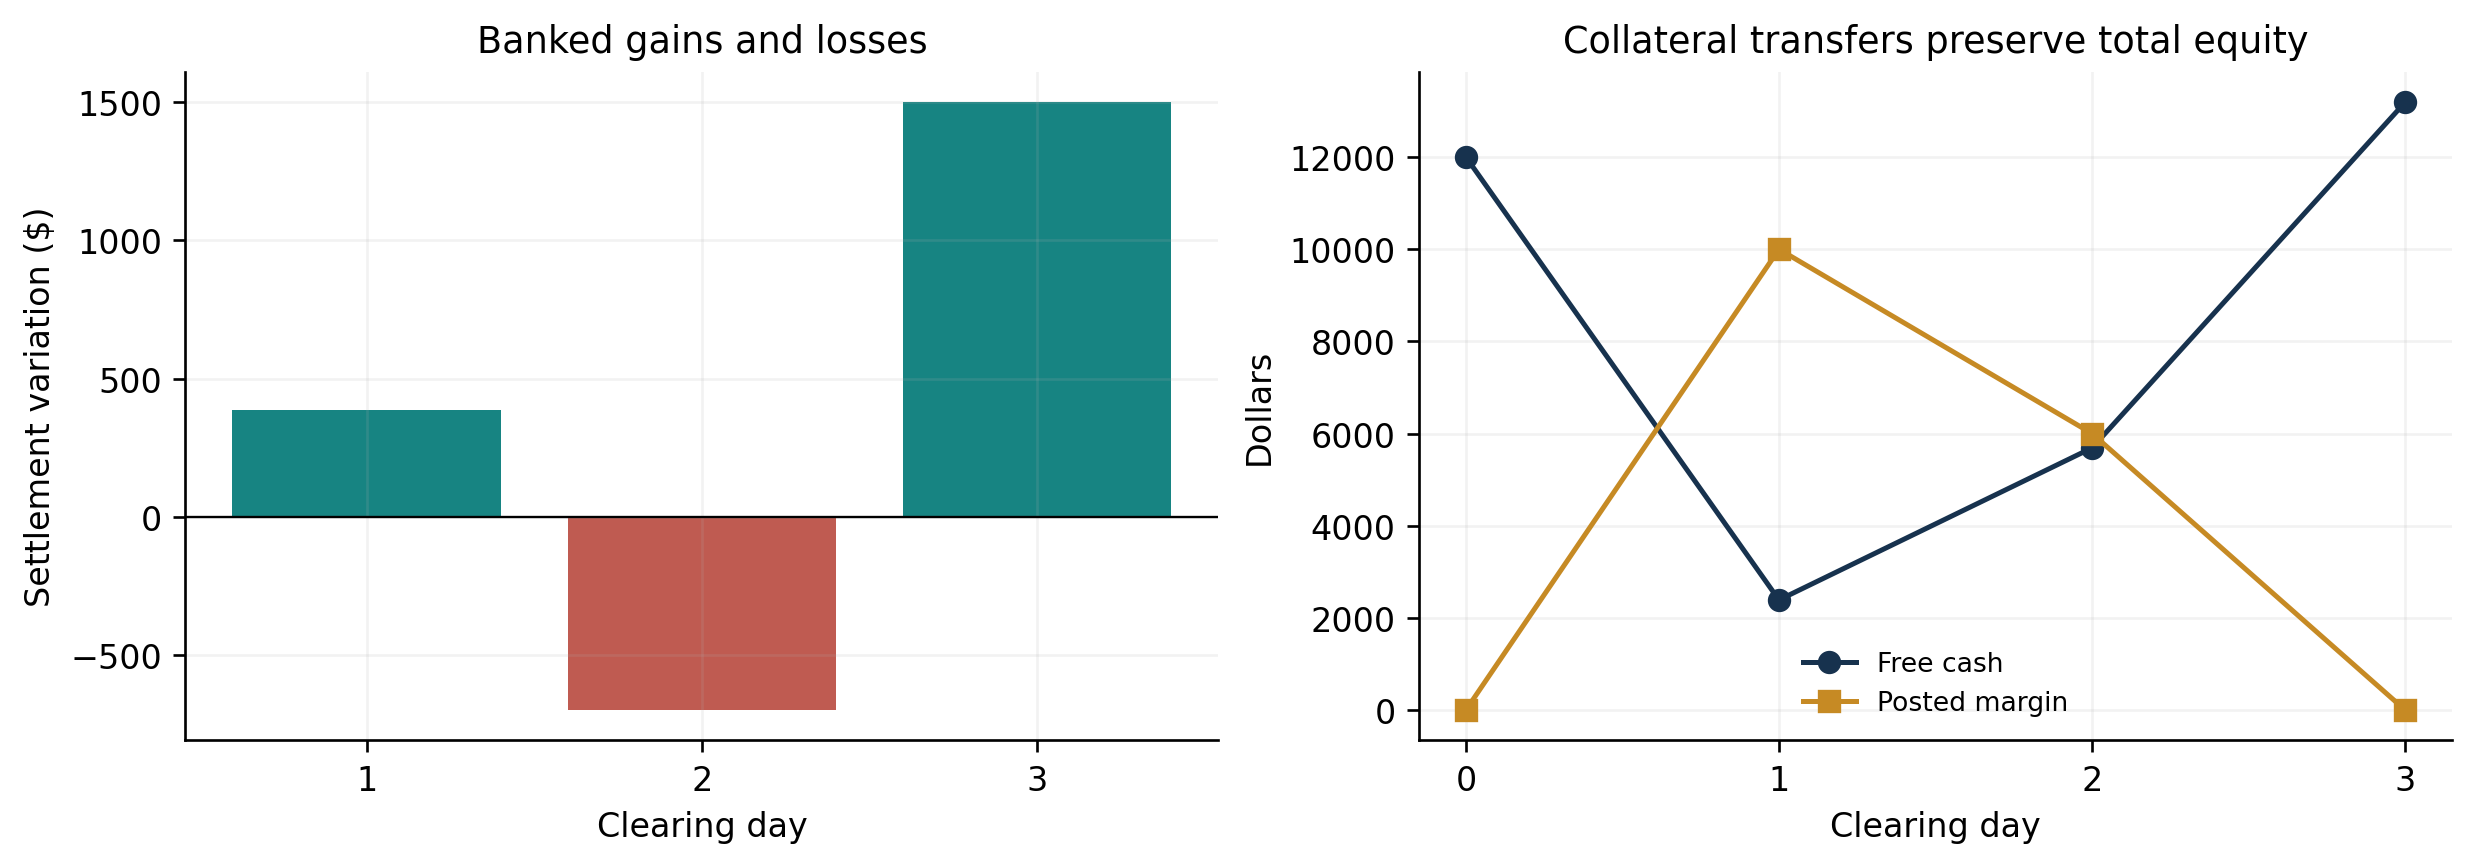
\includegraphics[width=\textwidth]{figures/06_settlement.png}
\caption{Cash flows and collateral in Table~\ref{tab:ledger}. Day 2 has negative variation but an increase in free cash because \$4,000 of posted margin is released. This is why a cash balance alone is not a P\&L series.}
\label{fig:ledger}
\end{figure}

The reconciliation uses the actual fills at their individual prices. Rounding the average fill to the nearest outright tick before calculating variation would alter the ledger. An average is a reporting summary; the trade records remain the accounting inputs.

\subsection{A default waterfall is another ordered allocation}

CME's public safeguards architecture places defaulter resources before the clearinghouse contribution, mutualized guaranty resources, and assessment powers \citep{CMESafeguards}. Account segregation and the applicable clearing service determine which resources are available. The following is an abstract loss-allocation model of that ordered structure, with no production dollar amounts or legal recovery rules inferred.

Let $L\ge0$ be a loss to absorb and $r_1,\ldots,r_k\ge0$ the resources available in the applicable order. Define
\begin{equation}
 d_i(L)=\min\left\{r_i,\left(L-\sum_{j<i}r_j\right)_+\right\},
 \qquad U(L)=\left(L-\sum_{i=1}^kr_i\right)_+.
\label{eq:waterfall}
\end{equation}

\begin{proposition}[Ordered loss conservation]
The draws in \eqref{eq:waterfall} satisfy $0\le d_i\le r_i$ and
\begin{equation}
 \sum_id_i(L)+U(L)=L.
\end{equation}
Each draw is continuous, nondecreasing, and piecewise linear in $L$. The first positive draw from layer $i$ occurs only after earlier resources are exhausted.
\end{proposition}
\begin{proof}
Represent each resource layer by a consecutive interval of length $r_i$. Its draw is the intersection length with $(0,L]$, exactly as in the FIFO prefix proof. The intersections partition the absorbed loss, and the portion beyond all intervals is $U(L)$.
\end{proof}

In synthetic millions of dollars, resources $(8,2,5,4)$ and loss 17 produce draws $(8,2,5,2)$ with no residual. The same arithmetic as FIFO appears because both allocate an amount through an ordered list of capacities. The economic interpretations differ: one allocates contracts to resting orders, the other losses to legally available resources.

Nominal capacity does not establish time availability. A future assessment may absorb an ultimate loss while failing to provide cash for an earlier settlement deadline. The funding theorem and the waterfall model therefore answer different questions: when cash is available, and whose resources absorb the loss.

\subsection{Reproducibility and the scope of verification}

The source project includes \texttt{reproduce.py} and nine PNG figures. Numerical outputs and runtime versions are recorded in \texttt{results.json} and \texttt{environment.json}. The script verifies 63 numerical result groups, including exact allocation vectors, the shared-capacity bound, opening cases, rounded values, the complete cash ledger, the margin counterexample, funding prefixes, option cash, delivery invoices, and waterfall draws. It also checks allocation conservation and discrepancy over 84 declared quantity, demand, and threshold combinations.

Fractions are used for proportional entitlements and price arithmetic; decimal arithmetic implements monetary rounding. A continuous linear program verifies the implied-resource upper bound, which is also certified analytically by Proposition~\ref{prop:dual}. All figures use deterministic synthetic inputs. There is no statistical fitting or Monte Carlo error.

These checks validate the published examples and modeled invariants. They do not certify product conformance, a live feed decoder, a production margin model, or a trading strategy. The source register identifies the operational documents and the part of each used in the manuscript.
\FloatBarrier
